\documentclass[aspectratio=169]{beamer}
%
% Choose how your presentation looks.
%
% For more themes, color themes and font themes, see:
% http://deic.uab.es/~iblanes/beamer_gallery/index_by_theme.html
%
\mode<presentation>
{
  \usetheme{metropolis}      % or try Darmstadt, Madrid, Warsaw, ...
  \usecolortheme{metropolis-imagelab} % or try albatross, beaver, crane, ...
  \usefonttheme{structurebold}  % or try serif, structurebold, ...
  \setbeamercolor{background canvas}{bg=white}
  \setbeamertemplate{navigation symbols}{}
  \setbeamertemplate{bibliography item}{\insertbiblabel}
  %\setbeamertemplate{caption}[numbered]
} 
\usepackage[english]{babel}
\usepackage[utf8x]{inputenc}
\usepackage{algorithm,algorithmic}
\usepackage{listings}             % Include the listings-package
\hypersetup{
    colorlinks = true,
    linkcolor = {black},
    urlcolor = {blue}
}

\DeclareMathOperator*{\argmin}{arg\,min}
\DeclareMathOperator*{\argmax}{arg\,max}

\title[Naive Bayes Classification]{Naive Bayes Classification}
\subtitle{Pattern Recognition and Machine Learning - MuMeT 2017}
\institute{University of Modena and Reggio Emilia}
\author{Davide Abati}
\date{October 12th, 2017}

\def\thisframelogos{}

\newcommand{\framelogo}[1]{\def\thisframelogos{#1}}

\begin{document}

\framelogo{logo_unimore_white.png}

\bgroup
\renewcommand{\insertframenumber}{}
\begin{frame}[noframenumbering]
  \titlepage
\end{frame}
\egroup
\bgroup
\begin{frame}{MNIST digits classification}
Today we meet MNIST for the first time:

\begin{minipage}{0.45\textwidth}
\centering
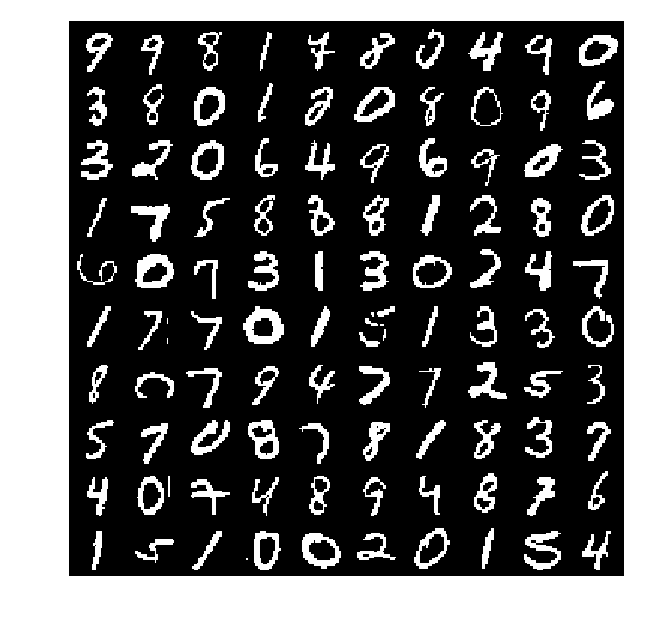
\includegraphics[width=\textwidth]{img/mnist.pdf}
\end{minipage}
\begin{minipage}{0.45\textwidth}
\begin{itemize}
\item 70000 images of handwritten images;
\item available grayscale, we will use a binarized version;
\item the task is to classify each image into the right digit.
\end{itemize}
\end{minipage}

\end{frame}
\egroup
\bgroup
\begin{frame}{Supervised learning setting}
We are given a training set $\{X_i, Y_i\}_{i=1}^n$, with $X_i \in \mathbb{R}^m$ and $Y_i \in \mathbb{R}$ for each $i=1,\ldots,n$.
\begin{itemize}
\item $n$ is the number of training images;
\item each image $X_i = \{x_i^{(1)}, \ldots , x_i^{(m)}\}$ is a vector of $m$ pixels;
\item each label $Y_i$ is just a number among $\{1, \ldots, d\}$.
\end{itemize}
\end{frame}
\egroup
\bgroup  
\begin{frame}{Classification using bayes rule}
We will use the Bayes rule to build a classifier. The classification rule will be the following:
\begin{equation*}
\argmax_Y \only<1,3,4,5>{P(Y/X)} \only<2>{\boxed{P(Y/X)}} = \frac{\only<1,2,3,5>{P(X/Y)}\only<4>{\boxed{P(X/Y)}} \only<1,2,4,5>{P(Y)}\only<3>{\boxed{P(Y)}}}{\only<1,2,3,4>{P(X)}\only<5>{\boxed{P(X)}}}
\end{equation*}
\begin{itemize}
\item<2-> $P(Y/X)$ is the probability of the image $X$ of being labeled as $Y$;
\item<3-> $P(Y)$ is the prior probability of the class $Y$;
\item<4-> $P(X/Y)$ is the likelyhood of the image $X$ under the model $Y$;
\item<5-> $P(X)$ is the probability of the image $X$ under the whole dataset. Does not influence the argmax so we can drop it.
\end{itemize}
\end{frame}
\egroup
\bgroup  
\begin{frame}{Prior $P(Y)$}
Finding the prior of a class $Y$ is easy.\\
Simply count the number of examples of each class and divide by the number of total examples.

\begin{equation*}
P(Y=c) = \frac{\sum_{i=1}^n \bold{1}\{Y_i == c\}}{n}
\end{equation*}
\end{frame}
\egroup
\bgroup  
\begin{frame}{Likelyhood $P(X/Y)$}
\textbf{Naive assumption}: all pixels are independent given the class. The probability of an image is the product of the probability of every single pixel.\\
\begin{equation*}
P(X_i/Y_c)=\prod_{j=1}^m P(x_i^{(j)}/Y_c)
\end{equation*}
During training, we need to model this for each possible class:
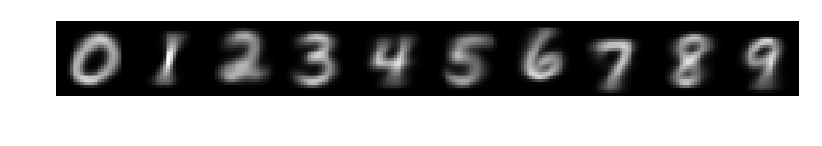
\includegraphics[width=\textwidth]{img/lkl_model.pdf}
\end{frame}
\egroup
\bgroup  
\begin{frame}{Likelyhood $P(X/Y)$}
During testing, the likelyhood of an image under a class is built by taking the class model (the one built before, during training) and:
\begin{itemize}
\item for each active pixel, account for the probability of being active given class;
\item for each zero pixel, account for one minus the probability of being active given class;
\end{itemize}
\begin{minipage}{0.25\textwidth}
\centering

\includegraphics[width=\textwidth]{img/test_image.pdf}
\end{minipage}
\begin{minipage}{0.65\textwidth}
\centering
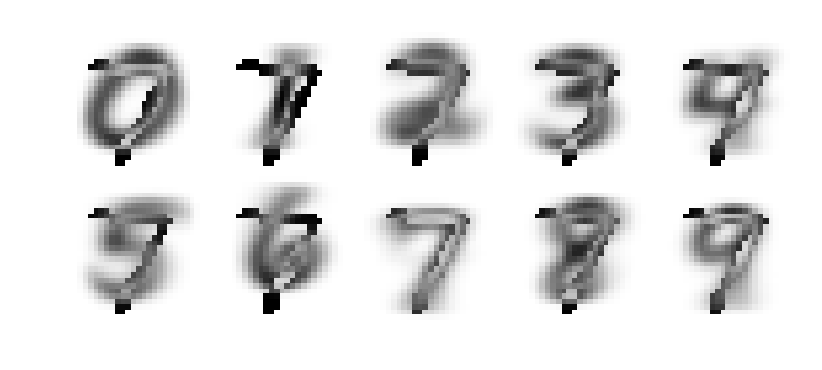
\includegraphics[width=\textwidth]{img/likelyhood.pdf}
\end{minipage}
\end{frame}
\egroup
%\bgroup  
\begin{frame}{Image probability $P(X)$}
It is computed the same way as the likelyhood, but estimating the model without conditioning on a particolar class.

Just use the whole dataset.
\end{frame}
\egroup
\bgroup  
\begin{frame}{Inference}
Once we can model $P(Y/X)$ for each class, we can classify an image by choosing the class that maximizes it:
\begin{equation*}
\tilde{Y} = \argmax_{Y} P(Y/X) = P(X/Y)P(Y)
\end{equation*}
\end{frame}
\egroup
\bgroup  
\begin{frame}{Use logarithms!}
All those products of probabilities can result in nothing. Use log-probabilities instead!
\begin{equation*}
\log{P(X_i/Y_c)}=\sum_{j=1}^m \log{P(x_i^{(j)}/Y_c)}
\end{equation*}
\begin{equation*}
\log{P(Y/X)} = \log{P(X/Y)} + \log{P(Y)}
\end{equation*}
\end{frame}
\egroup
\bgroup  
\begin{frame}{Wrap up: algorithms}
\begin{minipage}{0.45\textwidth}
\begin{algorithm}[H]
\begin{algorithmic}[1]
\FOR{$j=1$ to $d$}
\STATE compute the class prior $P(Y_j)$
\STATE compute a model for $P(X/Y_j)$
\ENDFOR
\end{algorithmic}
\caption{pseudocode for training}
\label{alg:train}
\end{algorithm}
\end{minipage}
\begin{minipage}{0.45\textwidth}
\begin{algorithm}[H]
\begin{algorithmic}[1]
\FOR{$i=1$ to $n$}
\FOR{$j=1$ to $d$}
\STATE compute $\log{P(X_i, Y_j)}$
\STATE compute $\log{P(Y_j/X_i)} = \log{P(X_i, Y_j)} + \log{P(Y_j)}$
\ENDFOR
\STATE $Y_i=\argmax_{Y_j}\log{P(Y_j/X_i)}$
\ENDFOR
\end{algorithmic}
\caption{pseudocode for inference}
\label{alg:test}
\end{algorithm}
\end{minipage}

\end{frame}
\egroup

\end{document}